\chapter{Proposed Solution Concept}
\label{chap:solution-concept}

To successfully fulfill the defined objectives, we propose the solution described in this chapter. We will develop a robust framework capable of generating semantic segmentation masks for individual TILs from weak bounding box annotations. The high-level overview of architecture can be seen in figure \ref{fig:sc-main}. It can be split into three main parts (modules) each responsible for different tasks:

\begin{enumerate}
    \item \textbf{Image preprocessing module} will contain various image preprocessing techniques, such as normalization of images.
    \item \textbf{Pseudo-label generating module} will be responsible for generating pseudo-labels in the form of segmentation masks.
    \item \textbf{Deep learning model} will use the preprocessed images and the generated pseudo-masks to make predictions.
\end{enumerate}

\begin{figure}[H]
    \begin{centering}
    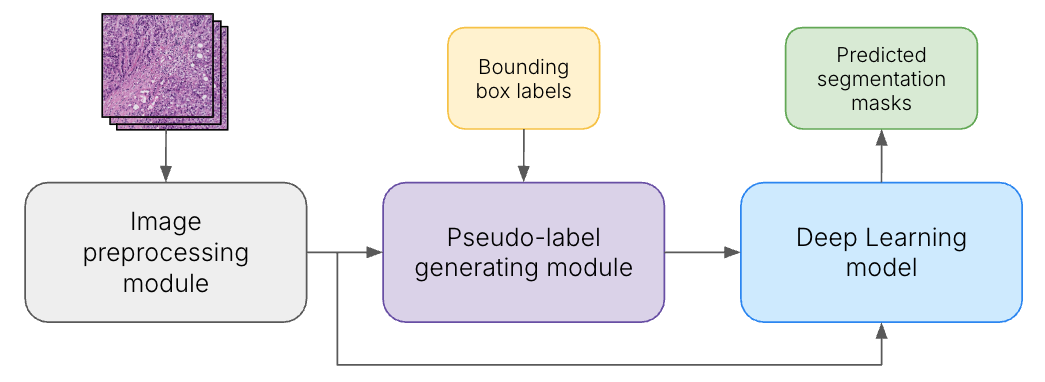
\includegraphics[width=14cm]{assets/images/sc-main.png}
    \par\end{centering}
    \caption{The high-level overview of the proposed architecture}
    \label{fig:sc-main}
\end{figure}

We describe each module in more detail in the following sections.

\section{Image Preprocessing Module}
This module will perform global preprocessing of images. Since the WSIs come from different institutes and different surgical procedures, normalization is a necessary step. We already performed the first experiments using Macenko normalization, and we mention these in the chapter \ref{chap:prelim-exp}.

The randomly selected image as a reference image for Macenko normalization laid suboptimal results. We have considered other approaches to selecting a reference image, but as a recent study \cite{Ivanov2024} showed when selecting only a single reference image for Macenko normalization, the results will always be biased and suboptimal. Therefore we would like to try experimenting with their proposed method of selecting multiple images to obtain better results. We would also like to try the normalization method used in \cite{Vahadane2015}, which showed promising results.

\section{Pseudo-label Generating Module}
The main task of this module will be the generation of pseudo-labels in the form of pixel-level masks. For this purpose, we crop out the individual cells with respect to their bounding box ground truth labels. Then we want to apply different traditional segmentation methods, such as GrabCut, watershed, and Otsu to obtain the mask for a single cell. We would also like to test tools such as QuPath and Cell Profiler as did authors in \cite{Zhang2022}. These individual masks will be then combined back into the large mask for the original large image. These large pseudo-masks will then be used by the deep learning model during training. The performance of these methods can be increased with different preprocessing techniques such as CLAHE or power law (gamma) transformation. This means that this module will also be responsible for some local image processing. We already performed preliminary experiments on this topic, which we write about in chapter \ref{chap:prelim-exp}.

\section{Deep Learning Model}
The final module will consist of a deep learning model. We would like to perform experiments with different architectures of CNN-based networks, and possibly Vision Transformers as well. We have not yet finalized the set of models we would like to experiment with but based on the related work, we consider U-Net-based architectures, namely Residual U-Net and Attention U-Net as our primary focus area. 

\section{Testing and Evaluation}
The evaluation metrics such as IoU and Dice score will be used for final evaluation and the best model will be selected and fine-tuned. The testing will need to be performed on a different dataset, which provides ground truth segmentation masks for TILs. The testing dataset is yet to be selected.
